\begin{frame}
	\frametitle{Bisimulations}
	\begin{itemize}[<+->]
		\itemspacing{20pt}
		\item Inspired by coinduction (Arbab et al.)
		\item Use bisimulations to reason about loops.
    \item Weak and strong bisimulations
    \item No correlation to transition systems
    \item Overapproximation and actual loop semantics
	\end{itemize}
\end{frame}

\begin{frame}
	\frametitle{Bisimulations}
	\begin{center}
		\includegraphics[height=\textheight]{semantics/img/weak_bisimulation.pdf}
	\end{center}
\end{frame}

\begin{frame}
	\frametitle{Bisimulations}
	\uncover<+->{
		\begin{definition}[Weak Bisimulation]
			Let $R$ be a binary relation.
			If $\pair{K, G} \in R$, then
			\begin{enumerate}[i)]
				\itemspacing{7pt}
				\item[] Let $G' = \wh(G)$
				\item $\resN{G'} \sqsubseteq K$
				\item $\pair{K - \resN{G'}, G'} \in R$
			\end{enumerate}
		\end{definition}
	}
	\uncover<+->{
		\begin{theorem}
			Let $R$ be a weak bisimulation.
			Then \[ \pair{K, G} \in R \land G \models B
			\implies \smtx{\while{B}{P}}(G) \sqsubseteq K \]
		\end{theorem}
	}
\end{frame}

\begin{frame}
	\frametitle{Bisimulations}
	\begin{center}
		\includegraphics[height=\textheight]{semantics/img/strong_bisimulation.pdf}
	\end{center}
\end{frame}

\begin{frame}
	\frametitle{Bisimulations}
	\uncover<+->{
		\begin{definition}[Strong Bisimulation]
			Let $R$ be a binary relation and $\varepsilon \in (0, 1)$.
			If $\pair{K, G} \in R$, then
			\begin{enumerate}[i)]
				\itemspacing{7pt}
				\item[] Let $G' = \wh(G)$
				\item $\resN{G'} \leqD K$
				\item $\pair{K - \resN{G'}, G'} \in R$
				\item $\left| \resN{G'}\right| \geq \varepsilon \cdot \l| K \r|$
			\end{enumerate}
		\end{definition}
	}
	\uncover<+->{
		\begin{theorem}
			Let $R$ be a strong bisimulation.
			Then \[ \pair{K, G} \in R \land G \models B
				\implies \smtx{\while{B}{P}}(G) = K \]
		\end{theorem}
	}
\end{frame}

\begin{frame}[fragile]
	\frametitle{Bisimulations}
	\begin{lstlisting}
 while (F = 0) {
   {X := X + 1}[0.5]{F := 1}
 }
	\end{lstlisting}
	\begin{itemize}[<+->]
		\itemspacing{10pt}
		\item $ G = 1$, $ K = \frac{1}{2 - X} $
		\item Bisimulation: $ R = \l\{ \pair{K, G}  \r\} \cup
			\only<+->{
				\l\{ \pair{
					\alert<+>{ \res{\frac{1}{2 - X}}{X \geq n} },
					\alert<+>{ \half^n \cdot \l( X^n F^0 + X^{n-1} F^1 \r) } } \ 
					\middle| \ n \in \N_{>0} \r\} 
			} $
		\item $R$ is in fact a strong bisimulation ($\varepsilon = \hf$)!
		\item $ \smtx{\while{F = 0}{\ldots}}(1) \sqsubseteq K $
		\item $ \smtx{\while{F = 0}{\ldots}}(1) = K $
	\end{itemize}
\end{frame}
